% A good introduction to latex can be found here:
%  http://www.cse.ohio-state.edu/~hank/latex/lshort141.pdf

\documentclass{article}
\usepackage{amsmath}

\usepackage{full page}  % make the margins somewhat smaller than the default

\usepackage{listings}  %  needed for source code listings
\usepackage{color}
\usepackage{hyperref}
\usepackage{graphicx}
\usepackage[tight,footnotesize]{subfigure}

\definecolor{javared}{rgb}{0.7,0,0} % for strings
\definecolor{javagreen}{rgb}{0.25,0.6,0.35} % comments
\definecolor{javapurple}{rgb}{0.55,0,0.40} % keywords
\definecolor{javadocblue}{rgb}{0.25,0.35,0.85} % javadoc
 
\lstset{language=Java,
basicstyle=\ttfamily,
keywordstyle=\color{javapurple}\bfseries,
stringstyle=\color{javared},
commentstyle=\color{javagreen},
morecomment=[s][\color{javadocblue}]{/**}{*/},
numbers=left,
numberstyle=\tiny\color{black},
stepnumber=2,
numbersep=10pt,
tabsize=4,
showspaces=false,
showstringspaces=false,
frame=shadowbox,
numbers=left
} 

% set the document title, author, and date here.
%  once set, the \maketitle command (within the document)
%  will display them nicely
\title{Mazeworld Solution}
\author{Junjie Guan $<gjj@cs.dartmouth.edu>$}

\begin{document}
\maketitle

\tableofcontents

\section{Introduction}

Sovling maze is one of the most classic and popular problems in Artificial Intelligence. This report majorly cover three parts, 1) indroducing the A* algorithm as a searching method; 2) Multirobot problem, where we need to take collision into consideration; 3) Blind robot problem, where the robot need to find out its current coordinate in the maze; 4) finally, some further discussion.

\clearpage
\section{A-star search}
\subsection{Basic Idea}

A* is a kind of informed search, which is different from traditional uninformed search (such as bfs). One huge difference is, instead of searching while trying to maintain as least cost as possible in bfs, A* also consider anohter value called heuristic. Figure \ref{astar} is a demostration of A* algorithm. On one hand, the solid line represent the path that we alredy go through, which is an evaluation of the past. On the other hand, the dash line, it represents the estimated/expected cost from current state to the goal, which is an evaluation of the future.

At every time A* pick the new state with lowest priority from a priority queue. Usually, it considers the past and the future simultaneously. Let's say the priority value is $f$, value of cost is $g$, and heuristic is $h$, then:
$$f = g + h$$

\begin{figure*}[!h]
\centering
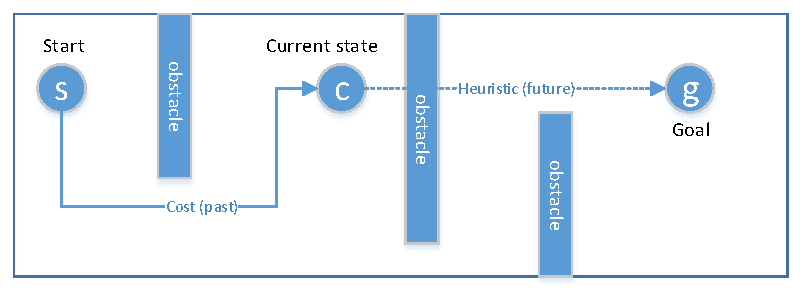
\includegraphics[width=0.927\textwidth]{astar.pdf}
\caption{A demostration of A* algorithm}
\label{astar}
\end{figure*}



\subsection{Single robot problem model}
The basic idea of single robot is to find a path from start position to the goal position. The state here is the coordinate of the robot, $(x,y)$.




\subsection{Code implementation}
\textbf{Line 3-7:} There are three major data structure to help me code astar.
\begin{itemize}
\item Priority queue: I use a priority queue to store the \emph{frontiers}, sorted by prioirty. Every search I will pop a node from the head of the queue.
\item Hash Map $\times 2$: One hashmap maps from node to node, for creating a backchain at the end. Another hashmap maps from node to priority, for the situation when we re-visit a node, it only worth expanding only if it has higher priority/cost than before.
\end{itemize}

\begin{lstlisting}[numbers=left]
public List<SearchNode> astarSearch() {
  resetStats();
  // implementing priority queue for the frontiers
  PriorityQueue<SearchNode> frontiers = new PriorityQueue<>();
  // implementing hashmap for the chain and the visited nodes
  HashMap<SearchNode, SearchNode> reachedFrom = new HashMap<>();
  HashMap<SearchNode, Double> visited = new HashMap<>();

  // initiate the visited with startnode
  reachedFrom.put(startNode, null);
  // initiate the frontier
  frontiers.add(startNode);
  while (!frontiers.isEmpty()) {
    // keep track of resource
    updateMemory(frontiers.size() + reachedFrom.size());
    incrementNodeCount();
    // retrieve from queue
    SearchNode current = frontiers.poll();
    // discard the node if a shorter one is visited
    if (visited.containsKey(current)
        && visited.get(current) <= current.priority())
      continue;
    else
      visited.put(current, current.priority());
    // mark the goal
    if (current.goalTest())
      return backchain(current, reachedFrom);
    // keep adding the frontiers and update visited
    ArrayList<SearchNode> successors = current.getSuccessors();
    for (SearchNode n : successors) {
      if (!visited.containsKey(n) || visited.get(n) > n.priority()) {
        reachedFrom.put(n, current);
        frontiers.add(n);
      }
    }
  }
  return null;
}
\end{lstlisting}

\textbf{Line 20-28:} After poping the node, we check for two condition. One is if it is the goal, we simply return the solution path and terminate the search. Antoher condition is, if the node has been visited before, we don't push it into \emph{frontiers} unless it has shorter cost than before.

\textbf{Line 29-35:} Get the successors of currrent node, and push those un-visited nodes or node has shorter cost than before, into the \emph{frontiers}.



\subsection{Output demonstration}



I use Simplex Noise to generate the maze.\footnote{I use authoried code from \url{http://webstaff.itn.liu.se/~stegu/simplexnoise/SimplexNoise.java to help me with the noise}} Figure \ref{s-1} shows a $40\times40$ maze, where all three robots try to move from bottom-left to middle-right. I leave the direction of robot at every single node. You can see that bfs and A* perform quite almost equally well, while dfs goes through a lengthy path.

The following output shows that, A* explored significantly less node than bfs, while the path length (cost) almost as less as bfs, while comparing to dfs.



\begin{lstlisting}[numbers=left]
BFS:
Nodes explored during search: 1064
Maximum space usage during search 1099
path length: 60
DFS:
Nodes explored during search: 399
Maximum space usage during search 242
path length: 242
A*:
Nodes explored during search: 79
Maximum space usage during search 224
path length: 72
\end{lstlisting}


\begin{figure*}[!h]
\centering
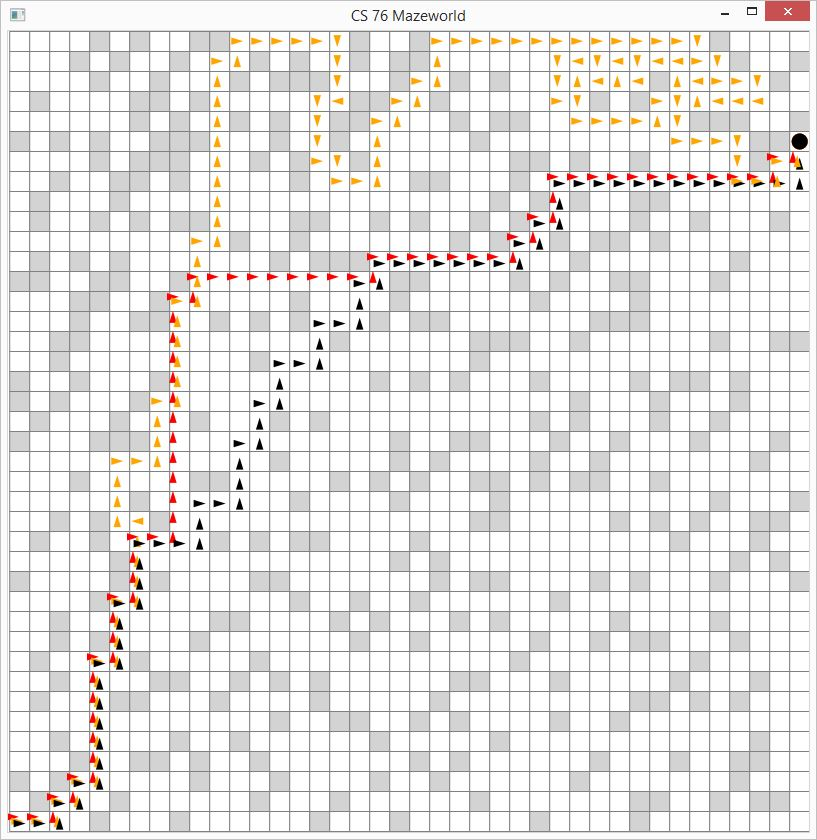
\includegraphics[width=0.618\textwidth]{s-1-1.JPG}
\caption{Searhing path of dfs(orange), bfs(red) and A*(black)}
\label{s-1}
\end{figure*}




\subsection{Discussion on cost and heuristic}
A* leverage both the cost (penalty) and the heuristic (search speed). Currently we use $f = h + g$ for priority, which seems quite a balanced solution. What happens if we go to extrem where the priority only related to $g$ or $h$? Or, is 50:50 the best choice for $f$?

Before I begin to discuss, I want to introduce a new kind of maze, where the obstacles can be crossed, while there is a certain amount of penalty. While I am first use Simplex Noise generate a maze, i replace the wall with number ranging from 1 to 10 to represent the weights. I use the following functions to differentiate nodes with different weights.
$$Grayscale = 255 - 255 \times weight / 20$$

Here I modify the expression of priority as following:
$$f = \alpha \cdot h + (1 - \alpha ) \cdot g$$
Then I vary $\alpha$ from 0 to 1, and observe their path length and cost. Figure \ref{s-2} shows the visual path with different configuration.
\begin{itemize}
\item Red ($\alpha = 0.0$) is an extreme case when A* only considers the cost, and becomes uninformed search. (I think it act like Dijkstra Algorithm). Since we are using Manhattan distance and the goal is at top-right, every action of moving south or west is a compromise of cost, and neglecting of path length ( search speed).
\item Brown ($\alpha = 1.0$) is another extreme case when A* only considers the heuristic, and becomes best-first search. We can observe that it totally neglect the cost/penalty, rushing to the goal in the simplest path.
\end{itemize}

Figure \ref{gh-plot} shows the change of path length and cost while varying $\alpha$. It depends on the tradeoff on searching speed and cost. It also greatly related to the problem definition, which affects the apperance of state space. For example, if path length and cost are on the scale $a : b$, then we should find $\alpha$, s.t. $min(a \cdot cost + b \cdot length)$.

\begin{figure*}[!h]
\centering
\includegraphics[width=0.628\textwidth]{astar_alpha.eps}
\caption{Plot describes the relationship between cost, path length, and $\alpha$}
\label{gh-plot}
\end{figure*}

\begin{figure*}[!h]
\centering
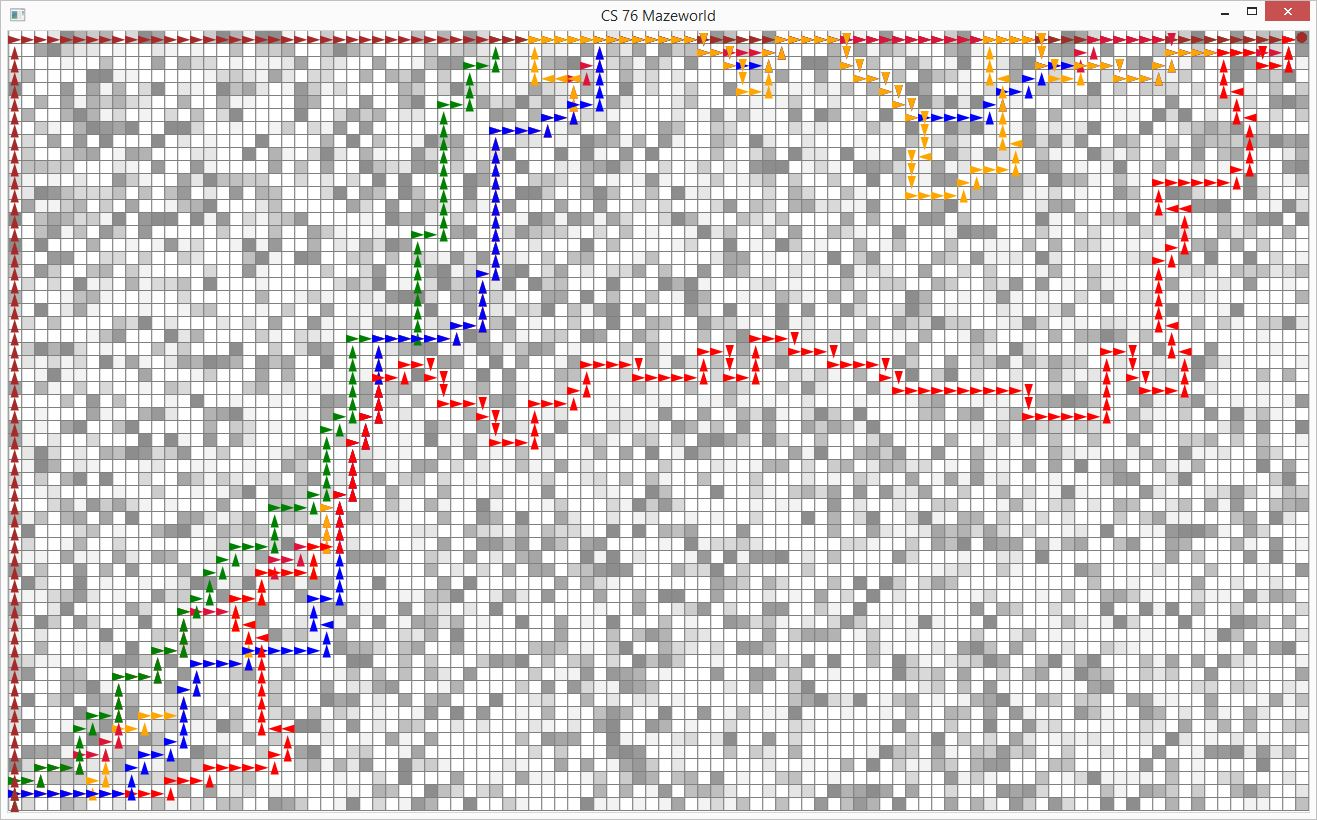
\includegraphics[width=1\textwidth]{s-2-1.JPG}
\caption{Varying the $\alpha$ in A* as 0.0 (red), 0.25 (orange), 0.5 (blue), 0.75 (crimson), 0.9 (green), 1.0 (brown)}
\label{s-2}
\end{figure*}






\clearpage
\section{Multirobot problem}
\subsection{Problem definition and states}

The different between single robot problem and multi robot problem is, every robot take turns to make actions, and it needs collision detection. In thiscase, we decide the a whole state for all the $k$ robots, like this:



$$\begin{pmatrix}
x_0 & y_0 \\
x_1 & y_1 \\
\vdots & \vdots \\	
x_{k-1} & y_{k-1}
\end{pmatrix}$$
However, this is not enough for the states. We still one parameter, which the turn of the robot. This parameter is not necessary, which means you can still solve the problem without it in the state. However, returning all the possible states of $k$ can be very redundant and time consumming for latter searching. If I have k robot, and five actions (4 directions plus not moving), the upper bound of states would be $5^k$. It is like giving too much options more next step, while I am not making any decision.











\subsection{Discussions}
ith $n\times n$ size of maze and $k$ robots, the upper bound of this problem, meaning to neglect the legal problem, is $n^{2k}$. Because each robot has $n$ possible position.

If number of wall square is $w$, then the number of collisions would be total state minus legal states, $(n^2-w)^k - C_{n^2-w}^k$. 

As for $100\times100$, with a few walls and several robot discussion. States number grows exponentially with $k$, and bfs tends to search all the state starting from start node. I think this problem still depends on whether the goal is close to the starting point.

As for the design of heuristic, I will use the following function,
$h = \sum^{k-1}_{i=0}h_i$, where $h_i$ represents the Manhattan distance from robot $i$ to the goal. A function is monotonic as long as\footnote{from \url{wiki: http://en.wikipedia.org/wiki/Consistent_heuristic}}:

$$h(N) \leq c(N,P)+h(P) $$
$$h(G)=0$$
where

\begin{itemize}
\item h is the consistent heuristic function,
\item N is any node in the graph,
\item P is any descendant of N,
\item G is any goal node,
\item c(N,P) is the cost of reaching node P from N.
\end{itemize}

It is obvious that for single robot, the single heuristic satisfy this condtions. An extreme case is the empty maze, where $h(N) = c(N,P)+h(P) $. In any other kind of maze, due to the obstacles, the $h$ usually larger than $cost$, because Manhattan distance is the shortest distance.

Under the condition that single heuristic satisfy this condtions. Adding them together should not affect the monotonicity.

The 8-puzzle problem is the case of multi-robot where there is no walls, and there is only one free space to move, and the goal is letting each robots move to its corresponding positions.

Whether 8-puzzle can be divided into two disjoint? This is similar to graph connectivity problem, or disjoint set problem. There is no better way but to traverse through all the possible states in 8 puzzle.

Let's say the total I calculate that the total states amount of this problem is $N$. My basic idea is, first I pick an arbitrary state, and use bfs to traverse all the connected states, push every one of them into a \textbf{hash set}. At this point the number of the set should be less then $N$. (Otherwise we turn out to prove there is no disjoint set.) Then I will pick antoher state that is not blong to the first set, and also use bfs to create another \textbf{hash set}. Finally, the sum of this two set should equal to $N$.



















\subsection{Code implementation}


\subsubsection{getSuccessors}

\textbf{getSuccessors} is used to expand new states from the current state.

\textbf{Line 4:} Iterate through all the 5 possible actions (4 directions plus not moving).
\textbf{Line 6-7:} Initiate the coordinates for the successor's state, noted that only the robot in turn can take action here.
\textbf{Line 11-13:} Construct the successor with new coordinates, and new cost based on whether it moves, and also keep looping the turn through $R$ robots.

\begin{lstlisting}[numbers=left]
public ArrayList<SearchNode> getSuccessors() {
  ArrayList<SearchNode> successors = new ArrayList<SearchNode>();
  Integer[] xNew = new Integer[R], yNew = new Integer[R];
  // take actions
  for (int[] action : actions) {
    for (int r = 0; r < R; r++) {
      xNew[r] = robots[r][0] + action[0] * (r == turn ? 1 : 0);
      yNew[r] = robots[r][1] + action[1] * (r == turn ? 1 : 0);
    }
    if (maze.isLegal(xNew[turn], yNew[turn])
        && noCollision(xNew, yNew)) {
      SearchNode succ = new MultirobotNode(xNew, yNew, getCost()
          + Math.abs(action[0]) + Math.abs(action[1]),
          (turn + 1) % R);
      successors.add(succ);
    }
  }
  return successors;
}
\end{lstlisting}


\subsubsection{noCollision}

\textbf{noCollision} is used to determine whether there is a collision of robots. I set it as private seems it is not used for outter class.

The basic idea is, I hash the position of each robot, and and check if the hash code already exists. If so, means there is another robot at this coordinate $(x,y)$; if not, push it into the hash set.

If I implement \textbf{noCollision} in simple iteration, the time complexity would be $O(k^2)$, while $k$ is the number of robots. By doing so, I reduce time complexity to $O(k)$.

\begin{lstlisting}[numbers=left]
private boolean noCollision(Integer[] xNew, Integer[] yNew) {
  HashSet<Integer> existed = new HashSet<>();
  for (int r = 0; r < R; r++) {
    Integer tmpHash = oneHash(xNew[r], yNew[r]);
    if (!existed.contains(tmpHash)) {
      existed.add(tmpHash);
    } else {
      return false;
    }
  }
  return true;
}
\end{lstlisting}




\subsubsection{Ohter methods}
Node constructor, it initiates the positions of robots iteratively.

\begin{lstlisting}[numbers=left]
public MultirobotNode(Integer[] x, Integer[] y, double c, int t) {
  robots = new int[R][2];
  for (int i = 0; i < R; i++) {
    this.robots[i][0] = x[i];
    this.robots[i][1] = y[i];
  }
  turn = t;
  cost = c;
}
\end{lstlisting}

Change the heuristic method to interative way.

\begin{lstlisting}[numbers=left]
public double heuristic() {
  // manhattan distance metric for simple maze with one agent:
  double hValue = 0;
  for (int i = 0; i < R; i++)
    hValue += Math.abs(xGoal[i] - robots[i][0])
        + Math.abs(yGoal[i] - robots[i][1]);
  return hValue;
}
\end{lstlisting}

\textbf{Line 20-28:} After poping the node, we check for two condition. One is if it is the goal, we simply return the solution path and terminate the search. Antoher condition is, if the node has been visited before, we don't push it into \emph{frontiers} unless it has shorter cost than before.

\textbf{Line 29-35:} Get the successors of currrent node, and push those un-visited nodes or node has shorter cost than before, into the \emph{frontiers}.



\subsection{Output demonstration}

Output of shifting 3 robots If we substract start and end, we know averagely every robot take 4 actions, that is acceptable in a wall-free space. (Figure \ref{m-1}):
\begin{lstlisting}[numbers=left]
A*:
path length: 14
Nodes explored during search: 167
Maximum space usage during search 577
\end{lstlisting}

Output of reodering robot in narrow corridor The path length is much longer that I expected. I guess it is because for an amount of time the robot just stay still, waiting for others. It is not easy to move in a narrow space. (Figure \ref{m-2}):
\begin{lstlisting}[numbers=left]
A*:
path length: 52
Nodes explored during search: 953
Maximum space usage during search 861
\end{lstlisting}


Output of cross road conflict. The average number of movements is 9, which is also reasonable. (Figure \ref{m-3}):
\begin{lstlisting}[numbers=left]
A*:
path length: 20
Nodes explored during search: 105
Maximum space usage during search 177
\end{lstlisting}

Output of moving relatively large number of robots. (Figure \ref{m-4}):
\begin{lstlisting}[numbers=left]
A*:
path length: 115
Nodes explored during search: 5070107
Maximum space usage during search 9081343
\end{lstlisting}

Output of moving relatively large maze. Noted that, although path length is much longer than the previous one, the explored nodes is actually much less. This is because states space size grow expoentially with number of robots. (Figure \ref{m-5}):
\begin{lstlisting}[numbers=left]
path length: 233
Nodes explored during search: 109132
Maximum space usage during search 184020
\end{lstlisting}


\begin{figure*}[!t]
% ensure that we have normalsize text
\normalsize
% Store the current equation number.
% Set the equation number to one less than the one
% desired for the first equation here.
% The value here will have to changed if equations
% are added or removed prior to the place these
% equations are referenced in the main text.
\centering
\subfigure[start]{
\label{m-1-3} %% label for first subfigure
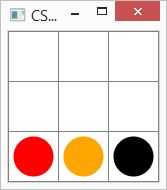
\includegraphics[width=0.16\textwidth]{m-1-3.JPG}}
\subfigure[step 1]{
\label{m-1-0} %% label for second subfigure
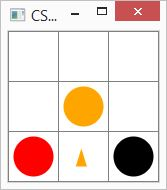
\includegraphics[width=0.16\textwidth]{m-1-0.JPG}}
\subfigure[step 2]{
\label{m-1-1} %% label for second subfigure
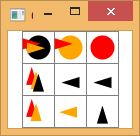
\includegraphics[width=0.16\textwidth]{m-1-1.JPG}}
\subfigure[step 3]{
\label{m-1-2} %% label for second subfigure
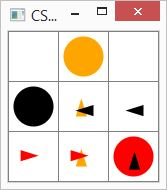
\includegraphics[width=0.16\textwidth]{m-1-2.JPG}}
\subfigure[end]{
\label{m-1-4} %% label for second subfigure
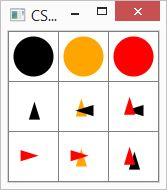
\includegraphics[width=0.16\textwidth]{m-1-4.JPG}}
\caption{Demo of shifting 3 robots}
\label{m-1} %% label for entire figure
\end{figure*}

\begin{figure*}[!t]
% ensure that we have normalsize text
\normalsize
% Store the current equation number.
% Set the equation number to one less than the one
% desired for the first equation here.
% The value here will have to changed if equations
% are added or removed prior to the place these
% equations are referenced in the main text.
\centering
\subfigure[start]{
\label{m-2-0} %% label for first subfigure
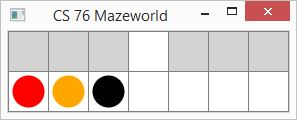
\includegraphics[width=0.206\textwidth]{m-2-0.JPG}}
\subfigure[step 1]{
\label{m-2-0} %% label for first subfigure
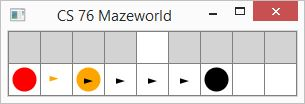
\includegraphics[width=0.206\textwidth]{m-2-1.JPG}}
\subfigure[step 2]{
\label{m-2-0} %% label for first subfigure
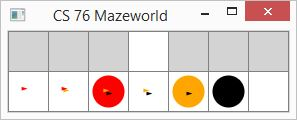
\includegraphics[width=0.206\textwidth]{m-2-2.JPG}}
\subfigure[step 3]{
\label{m-2-0} %% label for first subfigure
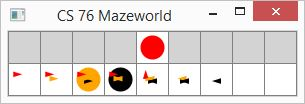
\includegraphics[width=0.206\textwidth]{m-2-3.JPG}}
\subfigure[step 4]{
\label{m-2-0} %% label for first subfigure
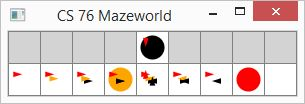
\includegraphics[width=0.206\textwidth]{m-2-4.JPG}}
\subfigure[step 5]{
\label{m-2-0} %% label for first subfigure
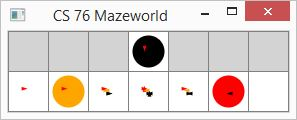
\includegraphics[width=0.206\textwidth]{m-2-5.JPG}}
\subfigure[step 6]{
\label{m-2-0} %% label for first subfigure
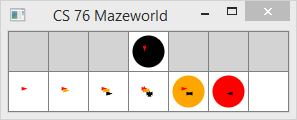
\includegraphics[width=0.206\textwidth]{m-2-6.JPG}}
\subfigure[end]{
\label{m-2-0} %% label for first subfigure
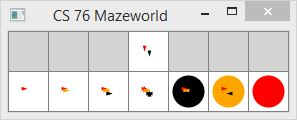
\includegraphics[width=0.206\textwidth]{m-2-7.JPG}}
\caption{Demo of reodering robot in narrow corridor}
\label{m-2} %% label for entire figure
\end{figure*}

\begin{figure*}[!t]
% ensure that we have normalsize text
\normalsize
% Store the current equation number.
% Set the equation number to one less than the one
% desired for the first equation here.
% The value here will have to changed if equations
% are added or removed prior to the place these
% equations are referenced in the main text.
\centering
\subfigure[start]{
\label{m-2-0} %% label for first subfigure
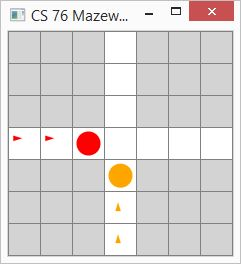
\includegraphics[width=0.206\textwidth]{m-3-0.JPG}}
\subfigure[step 1]{
\label{m-2-0} %% label for first subfigure
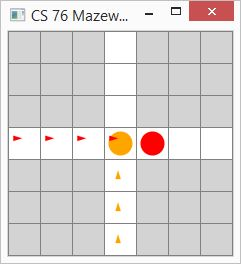
\includegraphics[width=0.206\textwidth]{m-3-1.JPG}}
\subfigure[end]{
\label{m-2-0} %% label for first subfigure
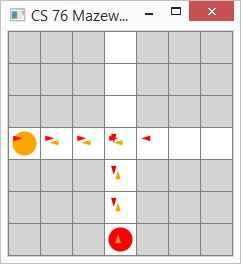
\includegraphics[width=0.206\textwidth]{m-3-2.JPG}}
\caption{Demo of cross road conflict}
\label{m-3} %% label for entire figure
\end{figure*}

\begin{figure*}[!t]
% ensure that we have normalsize text
\normalsize
% Store the current equation number.
% Set the equation number to one less than the one
% desired for the first equation here.
% The value here will have to changed if equations
% are added or removed prior to the place these
% equations are referenced in the main text.
\centering
\subfigure[start]{
\label{m-2-0} %% label for first subfigure
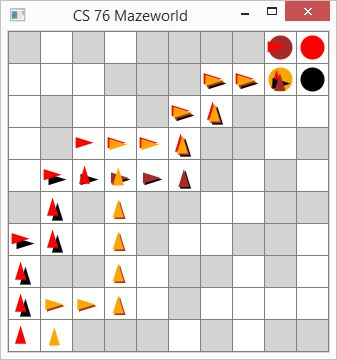
\includegraphics[width=0.618\textwidth]{m-4-1.JPG}}
\caption{Demo of moving relatively large number of robots}
\label{m-4} %% label for entire figure
\end{figure*}

\begin{figure*}[!t]
% ensure that we have normalsize text
\normalsize
% Store the current equation number.
% Set the equation number to one less than the one
% desired for the first equation here.
% The value here will have to changed if equations
% are added or removed prior to the place these
% equations are referenced in the main text.
\centering
\subfigure[start]{
\label{m-2-0} %% label for first subfigure
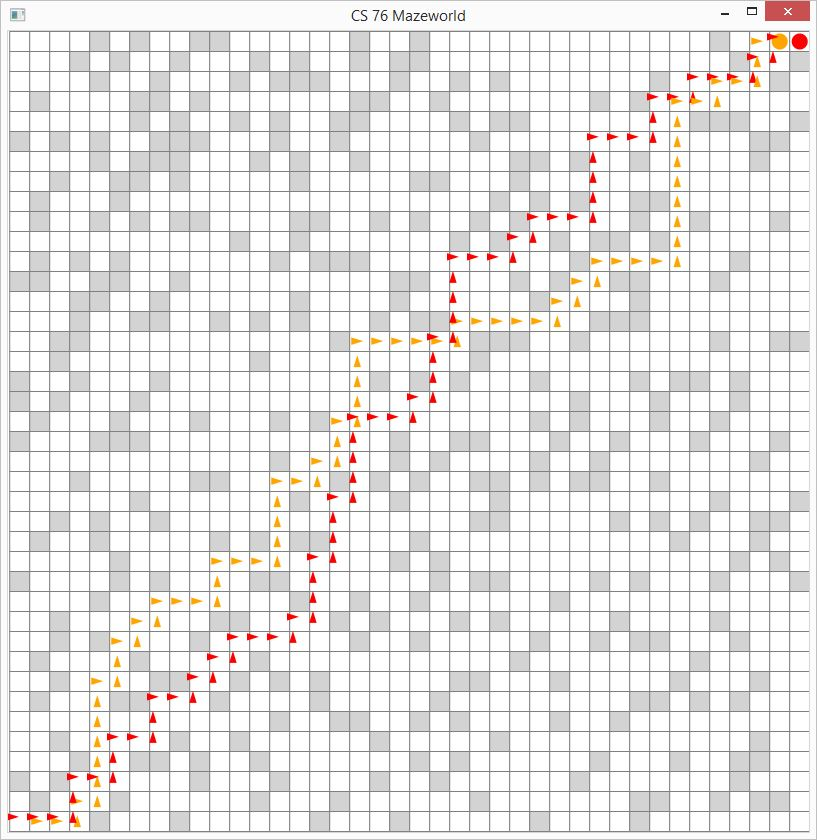
\includegraphics[width=0.818\textwidth]{m-5-1.JPG}}
\caption{Demo of moving relatively large large maze}
\label{m-5} %% label for entire figure
\end{figure*}






\clearpage
\section{Blind robot planning}
\subsection{Problem definition and states}

The basic idea is fill the maze with robots, give them instruction simultaneously, while gradually merging them to one point, which is the goal point.

The initial state looks similar to multi robot problem, which is also a 2-D matrix. $k$ equals to number of cell that is not wall.

$$\begin{pmatrix}
x_0 & y_0 \\
x_1 & y_1 \\
\vdots & \vdots \\	
x_{k-1} & y_{k-1}
\end{pmatrix}$$

The key of the problem is to design a consistent heuristic funciton. Which satisfy the formula in previous section. My intuition is approaching the goal while shrinking the range of robot positions. I think calculating the average and standard deviation of all the coordinates is a reasonable approach. The average describe the center of the group, the deviation describes the convergence. 

So, the state of this problem is as following, noted that $[x_i,y_i]$ is a $1\times 2$ matrix :
$$c_{x,y} = \sum^{k-1}_{i=0}[x_i,y_i]/k$$
$$d_{x,y} = ||\sqrt{ c_{x^2,y^2} - (c_{x,y})^2}||$$

Then, the heuristic function would be:
$$h =\textbf{max}(manhattan(c_{x,y}, g_{x,y}), d_{x,y})$$

How do I prove that the heuristic function is consistent? First, it apparently satisfy $h(G)=0$, because at that point, all robot will stay at one point, which makes $ d_{x,y} = 0$. Since the point is the goal, which makes, $manhattan(c_{x,y})=0$. As for $h(N) \leq c(N,P)+h(P) $, it is similar to the way that I used to prove monotonic previously. First let's assume an extreme case where there is an empty $N \times N$ maze, and the goal is at the top-right. I do a little math on it, it seems that if $N > 1 or N < -0.4$, the $cost$ is always larger than $h$. It is obvious always satisfied. (Since I must say I am not a mathematician, I'm not sure if I do it right, feel free to discuss with me if you doubt it).

\subsection{Discussions Polynomial-time blind robot planning}
If we take it as k-robot problem, where $k$ equals to number of cell. Then upper bound of the sates should be $(n-w)^k$. However, 

\subsection{Code implementation}

\subsubsection{getSuccessors}
Basic idea of \textbf{getSuccessors} is to move all robots with one action simultaneously. If there is obstacle for a robot, simply not moves. Note that at  \textbf{line 14}, the cost is the amount of robots that moves.
\begin{lstlisting}[numbers=left]
public ArrayList<SearchNode> getSuccessors() {
  ArrayList<SearchNode> successors = new ArrayList<SearchNode>();
  for (int[] action : actions) {
    HashSet<Coordinate> newCoords = new HashSet<>();
    // move all the node in the belief set to direction dxdy
    Coordinate dxdy = new Coordinate(action[0], action[1]);
    for (Coordinate xy : this.allCoord) {
      if (maze.isLegal(xy.x + dxdy.x, xy.y + dxdy.y)) {
        newCoords.add(new Coordinate(xy.x + dxdy.x, xy.y
            + dxdy.y));
      } else {
        // if not legal, simply not moving
        newCoords.add(new Coordinate(xy.x, xy.y));
      }
    }
    successors.add(new BlindRobotNode(newCoords, getCost() + 1.0
        * newCoords.size()));
  }
  return successors;
}
\end{lstlisting}


\subsubsection{Constructors}
The constructor is fairly simple. Note that, \textbf{line 14} is a very important methods, which is used to calculate the average cetner and deviation of all the coordinates. Some one might ask me why don't I compute the average and deviation while adding each new coordinate in the \textbf{getSuccessors}, so that everything can be done in one loop.  I got two reaons here. One is the time complexity is the same. The second is I want to keep the code simple, clean and modular. It is not just more easy to read and maintain, but also benifitial to the computing in the low level, since CPU don't have to access different address frequently.
\begin{lstlisting}[numbers=left]
public BlindRobotNode(HashSet<Coordinate> coords, double c) {
  // initiate the positions
  allCoord = coords;
  cost = c;
  newCenDev();
}

// dev = E(x^2) - (Ex)^2
private void newCenDev() {
  center = new Coordinate(0, 0);
  sDeviation = new Coordinate(0, 0);
  for (Coordinate xy : allCoord) {
    center.x += xy.x;
    center.y += xy.y;
    sDeviation.x += Math.pow(xy.x, 2);
    sDeviation.y += Math.pow(xy.y, 2);
  }
  center.x /= allCoord.size();
  center.y /= allCoord.size();
  sDeviation.x = Math.pow(sDeviation.x - center.x * center.x, 0.5);
  sDeviation.y = Math.pow(sDeviation.y - center.y * center.y, 0.5);
}
\end{lstlisting}


\subsubsection{newCenDev}

\textbf{newCenDev} creates the states, calculates the center and the deviation, for all the existing coordinate. Noted that the number of existing coordinate is decreasing, since some robots may merge together.
\begin{lstlisting}[numbers=left]
// dev = E(x^2) - (Ex)^2
private void newCenDev() {
  center = new Coordinate(0, 0);
  sDeviation = new Coordinate(0, 0);
  for (Coordinate xy : allCoord) {
    center.x += xy.x;
    center.y += xy.y;
    sDeviation.x += Math.pow(xy.x, 2);
    sDeviation.y += Math.pow(xy.y, 2);
  }
  center.x /= allCoord.size();
  center.y /= allCoord.size();
  sDeviation.x = Math.pow(sDeviation.x - center.x * center.x, 0.5);
  sDeviation.y = Math.pow(sDeviation.y - center.y * center.y, 0.5);
}
\end{lstlisting}

\subsubsection{Other methods}



The \textbf{heuristic} method.
\begin{lstlisting}[numbers=left]
@Override
public double heuristic() {
  // manhattan distance metric for simple maze with one agent:
  double dx = coordGoal.x - center.x;
  double dy = coordGoal.y - center.y;
  return Math.abs(dx) + Math.abs(dy) + sDeviation.x + sDeviation.y;
}
\end{lstlisting}










\subsection{Output demonstration}

Output of blind robot in 3x3. (Figure \ref{b-2}):
\begin{lstlisting}[numbers=left]
A*:  
  Nodes explored during search:  15
  Maximum space usage during search 100
  path length: 7
\end{lstlisting}

Output of blind robot in 7x7. (Figure \ref{b-2}):
\begin{lstlisting}[numbers=left]
A*:  
  Nodes explored during search:  15
  Maximum space usage during search 100
  path length: 7
\end{lstlisting}

\begin{figure*}[!t]
\normalsize
\centering
\subfigure[start]{
\label{b-1-0} %% label for first subfigure
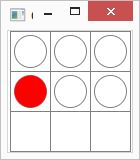
\includegraphics[width=0.206\textwidth]{b-1-2.JPG}}
\subfigure[step 3]{
\label{b-1-0} %% label for first subfigure
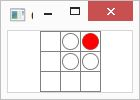
\includegraphics[width=0.206\textwidth]{b-1-3.JPG}}
\subfigure[step 4]{
\label{b-1-0} %% label for first subfigure
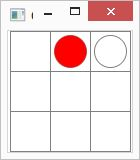
\includegraphics[width=0.206\textwidth]{b-1-4.JPG}}
\subfigure[step 5]{
\label{b-1-0} %% label for first subfigure
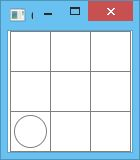
\includegraphics[width=0.206\textwidth]{b-1-5.JPG}}
\subfigure[step 6]{
\label{b-1-0} %% label for first subfigure
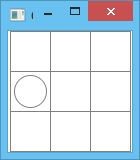
\includegraphics[width=0.206\textwidth]{b-1-6.JPG}}
\subfigure[end]{
\label{b-1-0} %% label for first subfigure
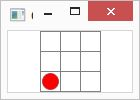
\includegraphics[width=0.206\textwidth]{b-1-7.JPG}}
\caption{Demo of blind robot in 3x3}
\label{b-1} %% label for entire figure
\end{figure*}

\begin{figure*}[!t]
\normalsize
\centering
\subfigure[start]{
\label{b-2-0} %% label for first subfigure
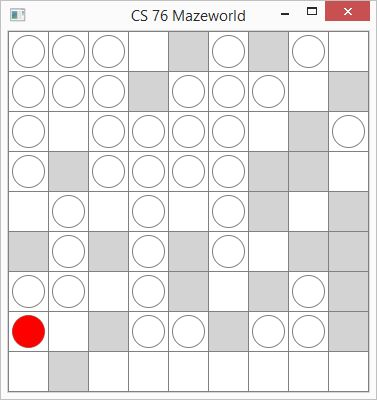
\includegraphics[width=0.206\textwidth]{b-2-2.JPG}}
\subfigure[step 3]{
\label{b-2-0} %% label for first subfigure
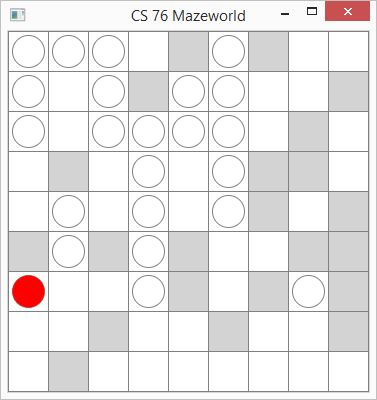
\includegraphics[width=0.206\textwidth]{b-2-3.JPG}}
\subfigure[step 4]{
\label{b-2-0} %% label for first subfigure
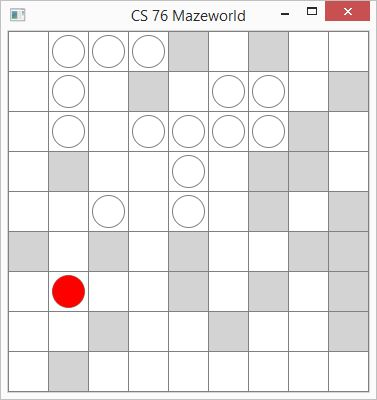
\includegraphics[width=0.206\textwidth]{b-2-4.JPG}}
\subfigure[step 5]{
\label{b-2-0} %% label for first subfigure
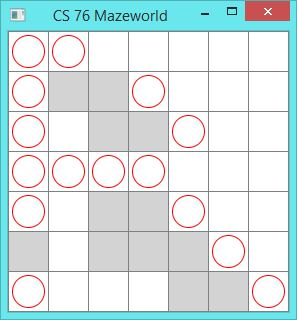
\includegraphics[width=0.206\textwidth]{b-2-5.JPG}}
\subfigure[step 6]{
\label{b-2-0} %% label for first subfigure
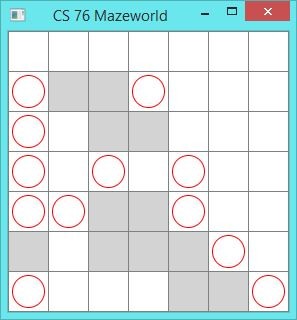
\includegraphics[width=0.206\textwidth]{b-2-6.JPG}}
\subfigure[step 7]{
\label{b-2-0} %% label for first subfigure
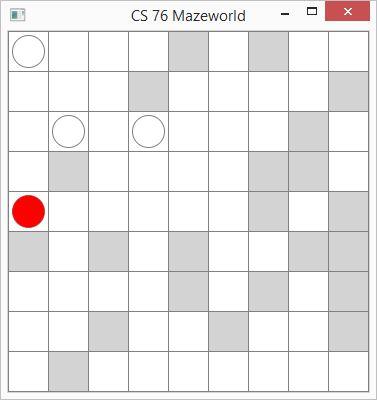
\includegraphics[width=0.206\textwidth]{b-2-7.JPG}}
\subfigure[step 7]{
\label{b-2-0} %% label for first subfigure
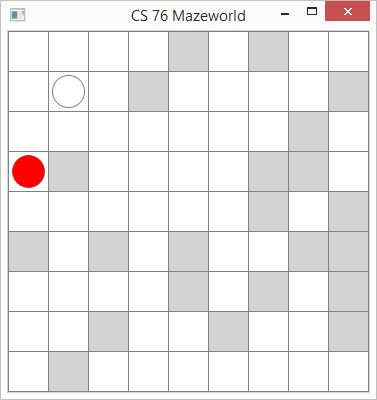
\includegraphics[width=0.206\textwidth]{b-2-8.JPG}}
\subfigure[step 7]{
\label{b-2-0} %% label for first subfigure
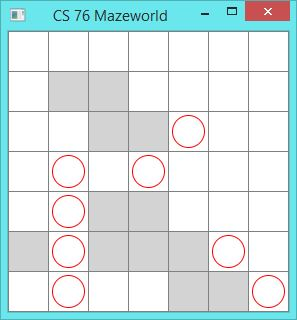
\includegraphics[width=0.206\textwidth]{b-2-9.JPG}}
\subfigure[step 7]{
\label{b-2-0} %% label for first subfigure
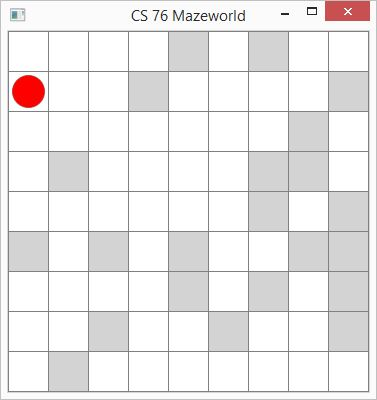
\includegraphics[width=0.206\textwidth]{b-2-10.JPG}}
\subfigure[step 11]{
\label{b-2-0} %% label for first subfigure
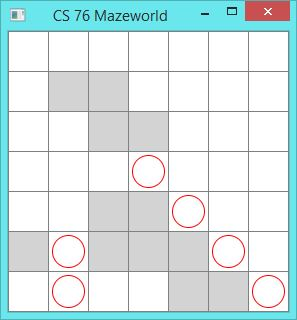
\includegraphics[width=0.206\textwidth]{b-2-11.JPG}}
\subfigure[step 12]{
\label{b-2-0} %% label for first subfigure
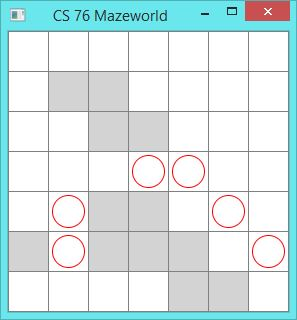
\includegraphics[width=0.206\textwidth]{b-2-12.JPG}}
\subfigure[step 13]{
\label{b-2-0} %% label for first subfigure
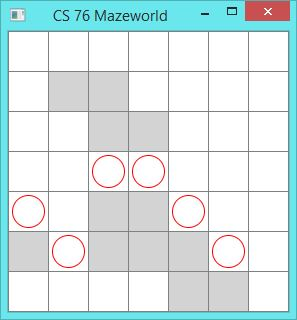
\includegraphics[width=0.206\textwidth]{b-2-13.JPG}}
\subfigure[step 14]{
\label{b-2-0} %% label for first subfigure
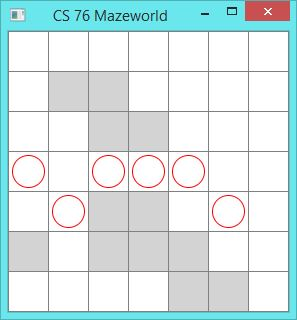
\includegraphics[width=0.206\textwidth]{b-2-14.JPG}}
\subfigure[step 15]{
\label{b-2-0} %% label for first subfigure
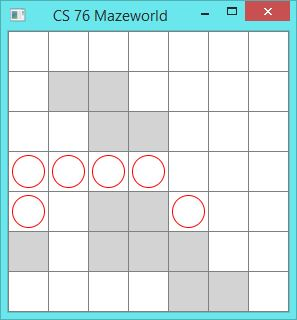
\includegraphics[width=0.206\textwidth]{b-2-15.JPG}}
\subfigure[step 16]{
\label{b-2-0} %% label for first subfigure
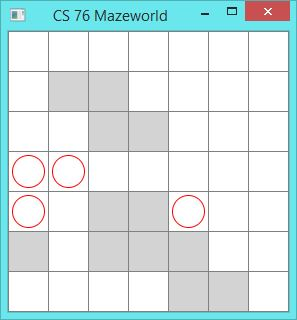
\includegraphics[width=0.206\textwidth]{b-2-16.JPG}}
\subfigure[step 17]{
\label{b-2-0} %% label for first subfigure
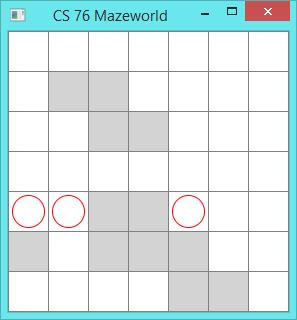
\includegraphics[width=0.206\textwidth]{b-2-17.JPG}}
\subfigure[step 18]{
\label{b-2-0} %% label for first subfigure
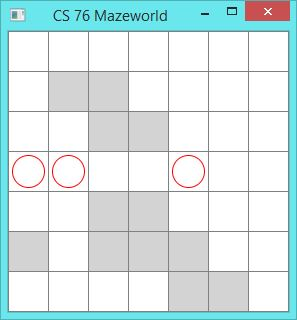
\includegraphics[width=0.206\textwidth]{b-2-18.JPG}}
\subfigure[step 19]{
\label{b-2-0} %% label for first subfigure
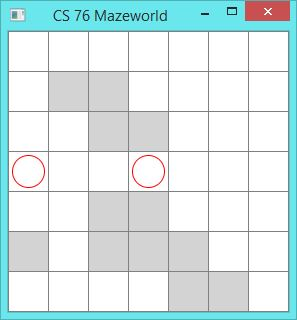
\includegraphics[width=0.206\textwidth]{b-2-19.JPG}}
\subfigure[step 20]{
\label{b-2-0} %% label for first subfigure
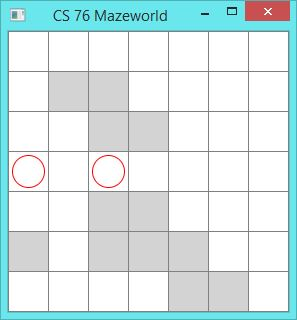
\includegraphics[width=0.206\textwidth]{b-2-20.JPG}}
\subfigure[step 21]{
\label{b-2-0} %% label for first subfigure
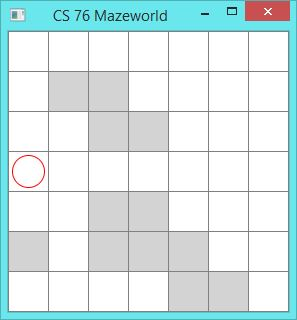
\includegraphics[width=0.206\textwidth]{b-2-21.JPG}}
\subfigure[step 22]{
\label{b-2-0} %% label for first subfigure
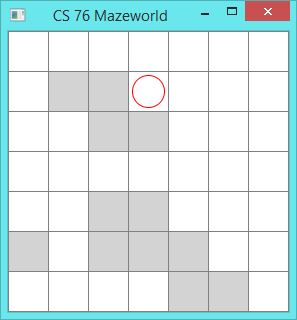
\includegraphics[width=0.206\textwidth]{b-2-22.JPG}}
\caption{Demo of blind robot in 7x7}
\label{b-2} %% label for entire figure
\end{figure*}
















\end{document}